\documentclass[12pt, a2paper]{article}
\title{Physics engine}
\author{Loi Yi Yang Caden}
\date{29 June 2023 - 31 December 2023}
\usepackage{graphicx}
\graphicspath{{images/}}

\begin{document}
\maketitle
\pagebreak

\tableofcontents
\pagebreak

\section{Purpose}
Physics engines are most commonly used for simulations of physics in games. However, there are also other purposes of a physics engine such as simulating systems that are hard or cannot be represented by an equation. This are systems like chaotic systems or systems where equation of acceleration cannot be integrated thus making it impossible to find the equation of velocities and displacements of a system. A physics engine, allows one to create a approximate of the velocities and displacement which can be represented in a graph or simply shown on a Graphical interface.

\section{How a physics engine works}
Physics engines have 3 essential components, a time step, a force generator and a ordinary differential equation solver(ODES).

\subsection{Time step}
A time step is one of the most important components of a physics engine as physics engine work by calculating the forces, velocities and displacements at every time step. The time step is the amount of time you "jump" in one interation, this means that you run the simulation after every time step. This means that the time step determinds how many iteration your programmes goes through and thus how long it takes to run, but at the same time also determinds the accuracy of the results.

\subsection{Force generator}
A force generator is a function that calculates the resultant force acting on an object at the time it is at. It does so by inputing known values such as the previous accleration, velocity, displacement of the object into equations which calculates what forces should be acting on it. 

This can be done by 2 major methods, the equation based method and the constraint based method.

The equation based method mostly gives you a more accurate calculation and is typically faster as it has a smaller time complexity. It is also simplier to implement as it does not usualy require multiple functions. However this method is restricted due to the need for the equation to be manually calculated and thus makes it difficult to have very complex simulations with multiple objects.

The constraint based method uses the concept of constraints. For example a rigid body in 2D has 3 degrees of freedom, 2 positional and 1 rotational. A constraint decreases the degrees of freedom of an object. For instance, a constraint that pins an object in space at its center of mass decreases the object’s degrees of freedom by 2 as all the positional degrees of freedom are removed and the object can thus now only rotate with 1 degrees of freedom.

In a constraint based physics engine, everything is modled as a constraint including collision contacts, frictions, springs, pulleys. This works by using constrains to solve interactions between 2 or more bodies.

\subsection{Ordinary differential equation solver(ODES)}
A ODES is a fucntion that calculates the value of the integrated equation at a time step using an approximation to allow you to find an approximation of the velocity and displacement of an object at each time step. This can be done by 2 main methods. Euler forward differencing which is a simpler but more unstable method, and Runge Kutta which has a fourth order method. 

\subsubsection{Euler forward differencing method}
Euler forward differencing method works simply by taylor expanding the ordinary differencial equation (ODE) and then multipling it by the time step (Marenduzzo). However, it's accuracy is also directly correlated to how small the time step is. This forces the timestep to be very small for you to get an accurate result, this slows down the simulation and makes it more complex. 

\subsubsection{Runge Kutta Fourth order method(RK4)}
RK4 uses 4 estimates of the derivatives and takes the a weighted average of these derivatives. The four derivatives are given by the below equations where \(t\) is the total time, \(y\) is a inital condition that is to be updated and \(h\) is the time step. 
\[k_{1} = f(t,y)\]
\[k_{2} = f(t+\frac{h}{2},y+h\frac{k_{1}}{2}\]
\[k_{3} = f(t+\frac{h}{2},y+h\frac{k_{2}}{2}\]
\[k_{4} = f(t+h,y+hk_{3})\]

This gives a good approximation up to the fourth order and does not require you to run at a very low time step.

\section{Example simulations}
\subsection{Terminal velocity of a ball}
A simple simulation to show test and show how the physics simulator works is through simluting the terminal velocity of a ball.

This is a fairly simple simulation as it only works in one dimension.

The equation of resultant force can be given by adding the weight, bouyancy force and air resistance, which can be given by these equation, where \(m\) is the mass, \(g\) is the gravitational acceleration constant, \(r\) is the radius of the ball, \(\rho\) is fluid density, \(v\) is current velocity of the ball and \(c\) is the drag coefficient.
\[weight = mg\]
\[air\:resistance = \frac{1}{2}\rho v^2 c\cdot 2\pi r^2\]
\[bouyancy = -\rho g \cdot\frac{4}{3}\pi r^3\]

This can then be added and divided by the mass to find the accleration of the ball.

This can then simply be called at each iteration and run through a ODES to find the velovity and then once again to find the position.

I then output this into a Comma seperated values(CVS) file and create the graph using excel.
\begin{figure}[h]
\centering
\includegraphics[width=1\textwidth]{ball terminal velocity function}
\caption{Code implementing ball terminal velocity}
\label{fig 1}
\end{figure}
\begin{figure}[h]
\centering
\includegraphics[width=1\textwidth]{ball terminal velocity graph}
\caption{Graph from ball terminal velocity function}
\label{Graph 1}
\end{figure}

In Figure \ref{Graph 1} series 1 is the x-componet of velocity, series 2 is the y-component of velocity, series 3 is the x-component of displacement and series 4 is the y-component of displacement.
\pagebreak

\subsection{Thrown ball}
To take the engines abilities to the next step we make it so that it can simulate in 2 dimensions. We can test and demonstrate this by simulating a thrown ball.

To simulate in 2 dimension, we need to have a way to store and add vectors. I stored by vector by using a pair of pairs. The first pairs stores the vector like cartesian coordinates by storing the x and y component. the second pair stores the vector like polar coordinates storing the magnitude and direction of the vector.
\begin{figure}[h]
\center
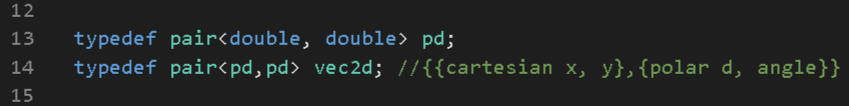
\includegraphics[width = 1\textwidth]{vec2d definition}
\caption{Defining 2D vectors}
\label{fig 2}
\end{figure}
\pagebreak

There is minimal changes needed to be done to the force generator and the ODES which ainly include changing what value types the function takes in.

Then we can run the programme again after adding initial velocities to simulate a thrown ball.
\begin{figure}[h]
\center
\includegraphics[width=1\textwidth]{thrown ball function}
\caption{Code implementing a thrown ball}
\label{fig 3}
\end{figure}
\begin{figure}[h]
\center
\includegraphics[width=1\textwidth]{thrown ball graph}
\caption{Graph from thrown ball function}
\label{Graph 2}
\end{figure}

In Figure \ref{Graph 2} , series 1 is the x-componet of velocity, series 2 is the y-component of velocity, series 3 is the x-component of displacement and series 4 is the y-component of displacement.
\pagebreak

\subsection{Single pendulum}
In order to demonstrate how the physics engine simulates a system with angular velocity, we can use a simulation of a simple pendulum. 

To simplify the calculations for angular accleration, we can use a lagrangian to solve it instead. We can start create this lagrangian by defining the constraints of the x and y displacements of the bob.
\[x = lsin\theta\]
\[y = -lcos\theta\]

We can then use the first derivitives of this coordinates with respect to time \(\dot{\vec{X}} = l\dot{\vec{\theta}}cos\theta\) and \(\dot{Y} = l\dot{\theta}cos\theta\) to find the Kinetic energy.
\[Ke = \frac{1}{2}mv^2\]
\[= \frac{1}{2}m(l^2\dot{\theta}^2(cos\theta)^2+l^2\dot{\theta}^2(sin\theta)^2)\]
\[\frac{1}{2}ml^2\dot{\theta}^2\]

The lagragian will then be,
\[L = \frac{1}{2}ml^2\dot{\theta}^2-mg(l+y)\]
\[= \frac{1}{2}ml^2\dot{\theta}^2-mgl+mglcos\theta\]

Now that we have the lagrangian we can use Eular's lagrange equation \(\frac{dp\theta}{dt}-\frac{\partial L}{\partial\theta} = 0\) to find the angular acceleration.
\[ml^2\ddot{\theta}+mglsin\theta\]
\[\ddot{\theta} = \frac{-gsin\theta}{l}\]

The are no changes to be made to the ODES and we can simply run the function to simulate the simple pendulum.
\begin{figure}[h]
\center
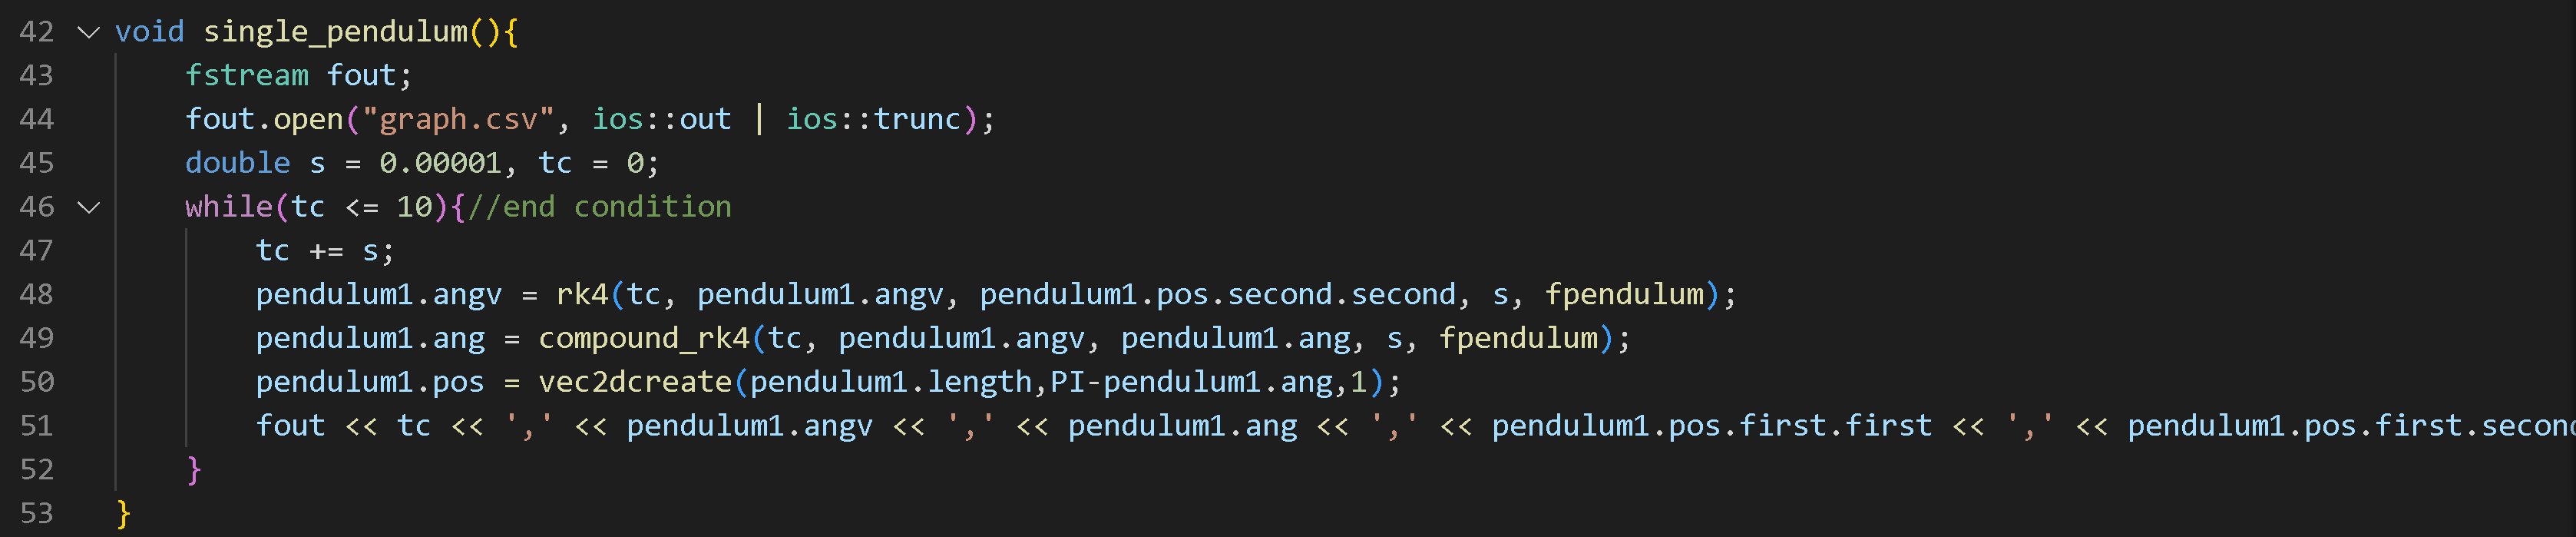
\includegraphics[width=1\textwidth]{Simple pendulum function}
\caption{Code implementing a simple pendulum}
\label{fig 4}
\end{figure}
\begin{figure}[h]
\center
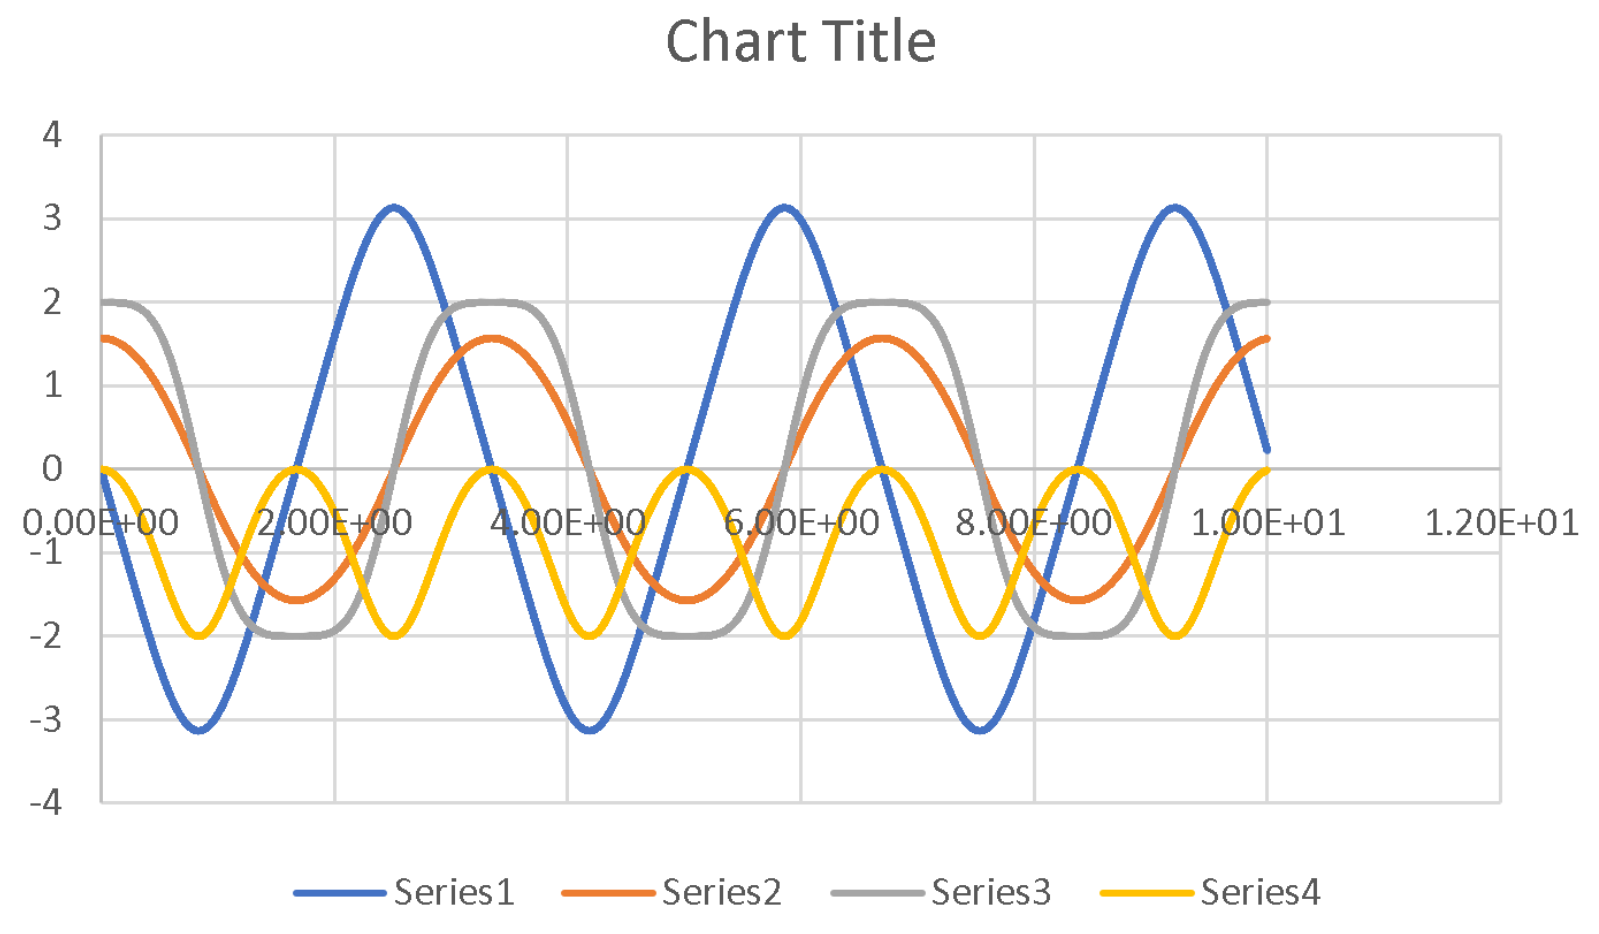
\includegraphics[width=1\textwidth]{Simple pendulum graph}
\caption{Graph from simple pendulum fucntion}
\label{Graph 3}
\end{figure}
\pagebreak

In Figure \ref{Graph 3}  below, series 1 is the angular velocity, series 2 is the angle from the center, series 3 is the x-component of displacement and series 4 is the y-component of displacement.

One interesting thing we can use this for is to show how the small angle aproximation equation of period of a simple pendulum becomes in accurate when the initial angle becomes to big. 

This is something that can also be observed in the derivation of this formular as it makes and assumtion that \(sin\theta = \theta\) which is only true for very small values.

We can show this by creating a condition so that the programe will output the time after it makes one oscillation. We can then iterate through many initial angles to create a graph. This can then be compared with the equation to show that the period changes when the intial angle is increased unlike what the equation suggest.
\begin{figure}[h]
\center
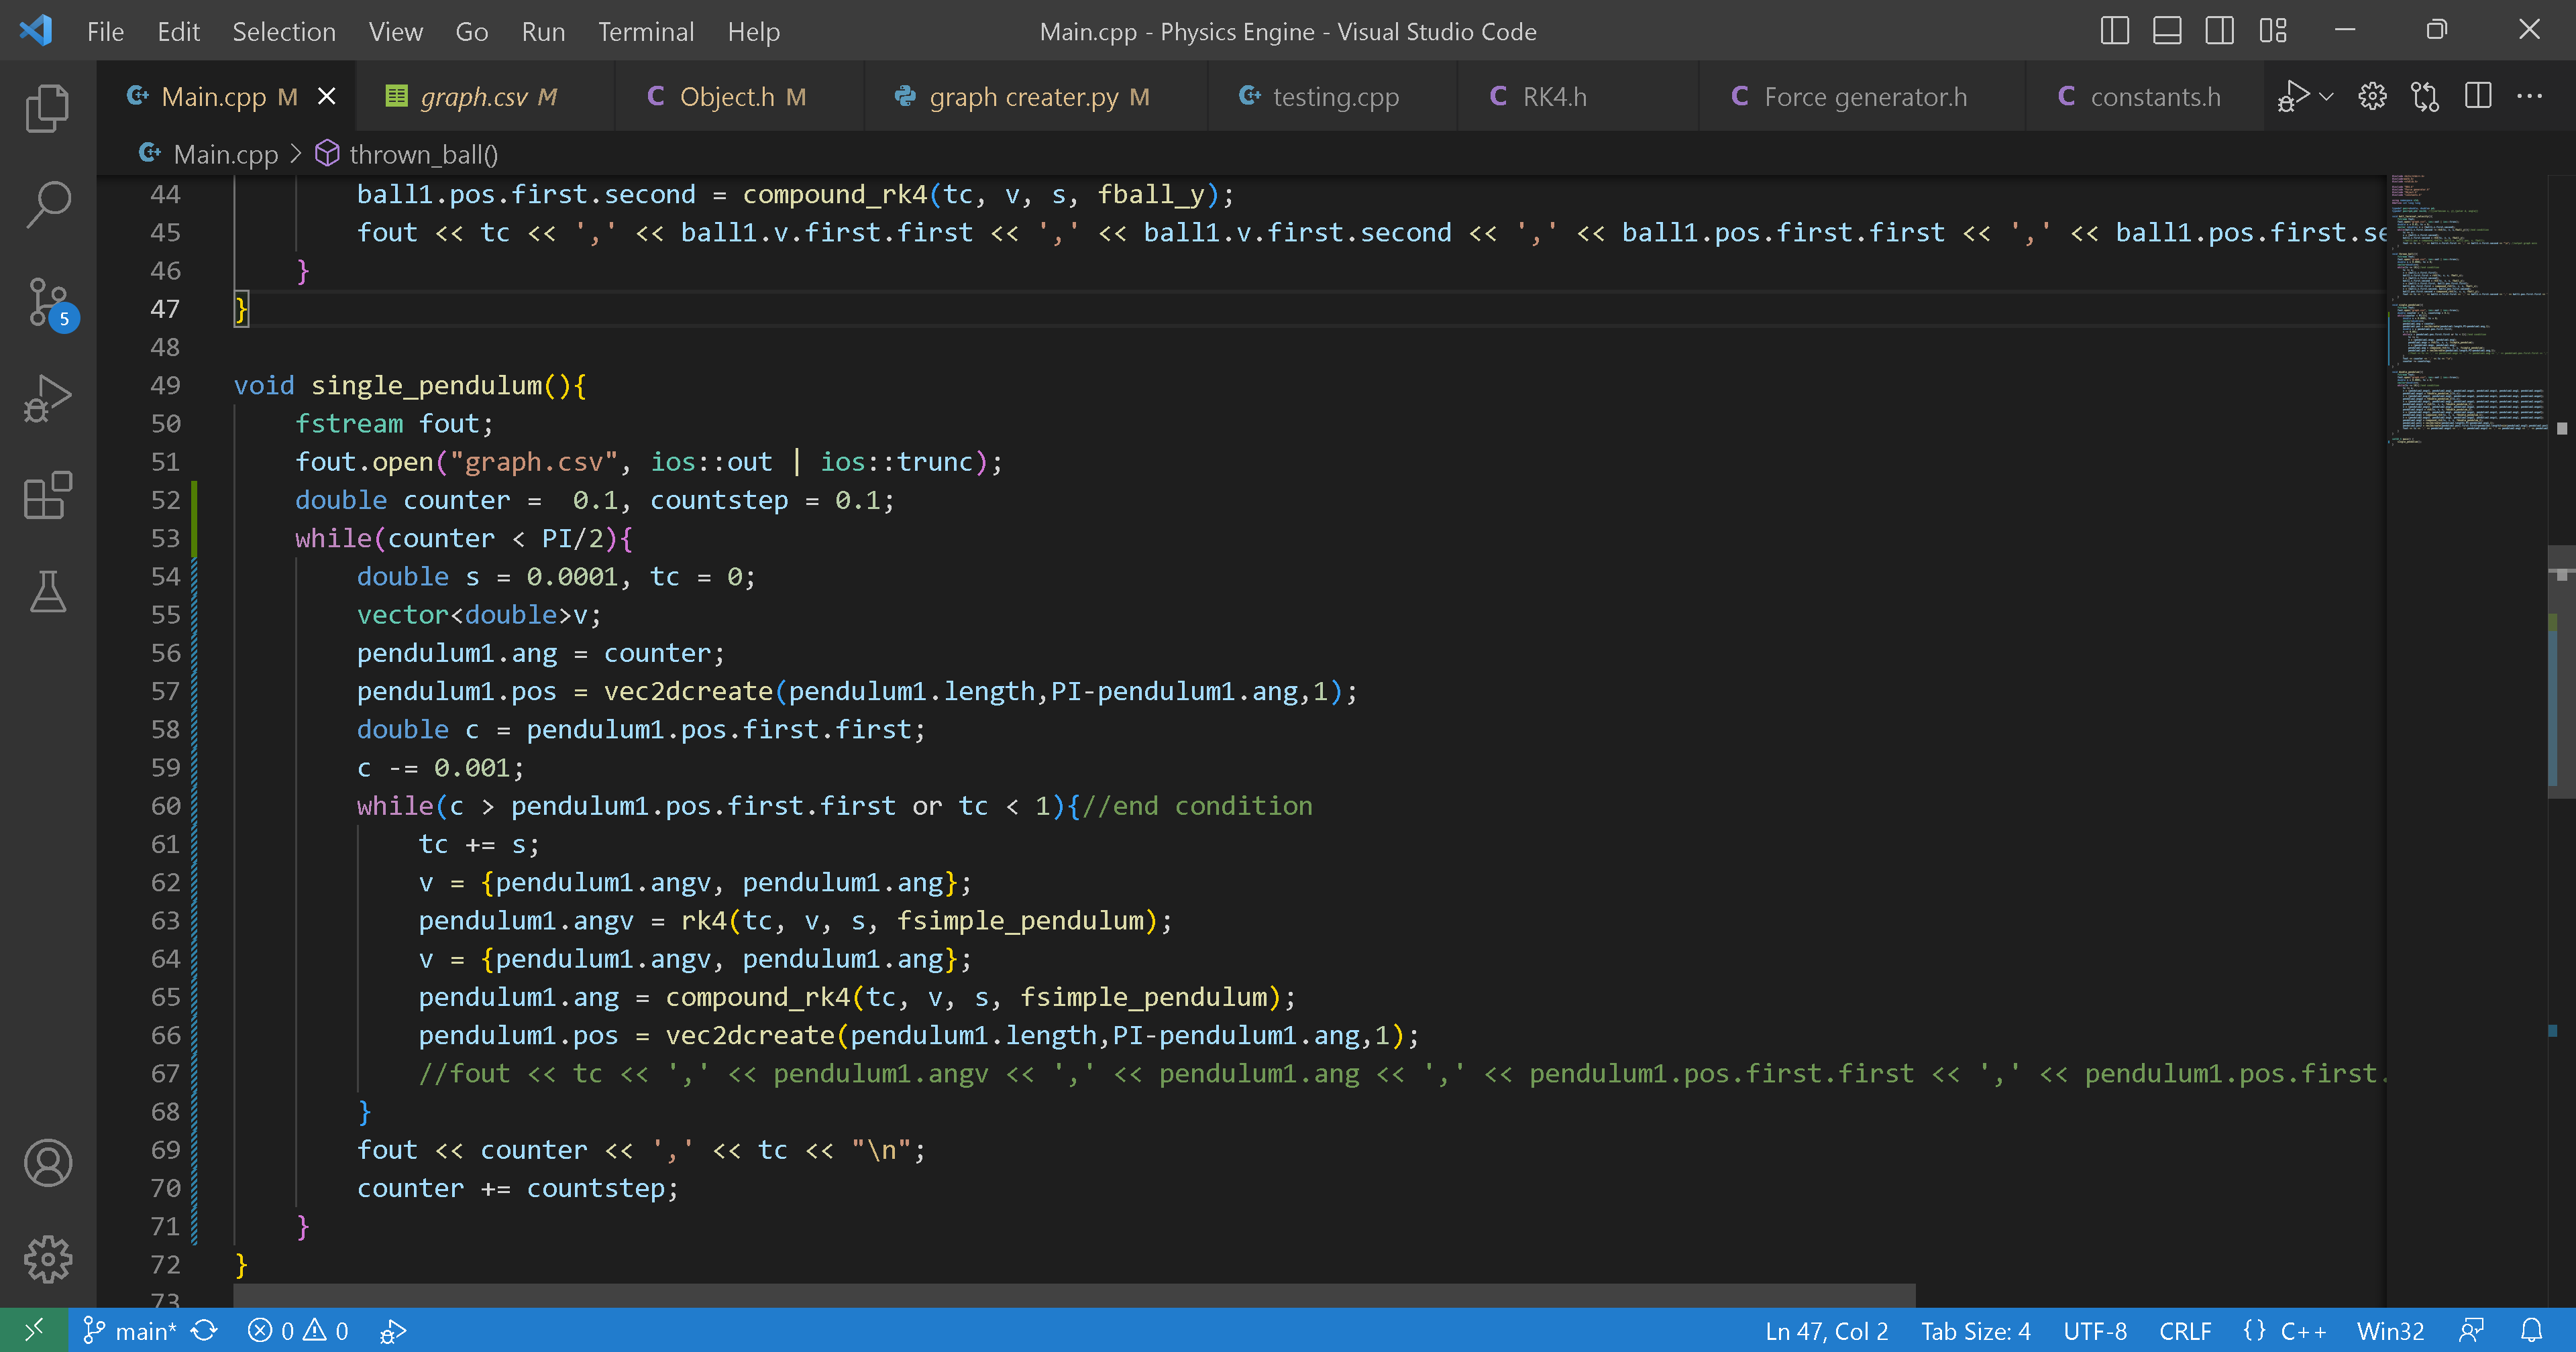
\includegraphics[width=1\textwidth]{Period of pendulum function}
\caption{Code implementing the period of a simple pendulum}
\label{fig 5}
\end{figure}
\begin{figure}[h]
\center
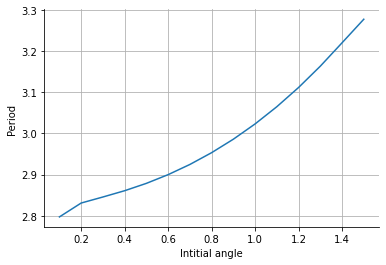
\includegraphics[width=1\textwidth]{Period of pendulum graph}
\caption{Graph from period of simple pendulum fucntion}
\label{Graph 4}
\end{figure}

From Figure \ref{Graph 4} we can see that the equation slowly becomes more and more inaccurate as the initial angle increases and becomes very inaccurate by 1dp at an initial angle of 1 radian.

It is also worth noting that exel, which i was using to plot my graphs became very slow as the amount of values increased, so i created a python programme to plot the graph suing matplotlib instead.
\pagebreak

\subsection{Double pendulum}
Another interesting simulation we can do is a double pendulum. This is interesting as it demonstrates that physics engine can simulate choatic systems.

We can start doing this by solving a lagrangian as it would be much simpler then solving using newtonian mechanics.
\[x_{1} = l_{1}sin\theta_{1}\]
\[y_{1} = -l_{1}cos\theta_{1}\]
\[x_{2} = l_{1}sin\theta_{1}+l_{2}sin\theta_{2}\]
\[y_{2} = -l_{1}cos\theta_{1}-l_{2}cos\theta_{2}\]
\[\dot{x}_{1} = l_{1}\dot{\theta}_{1}cos\theta_{1}\]
\[\dot{y}_{1} = l_{1}\dot{\theta}_{1}sin\theta_{1}\]
\[\dot{x}_{2} = l_{1}\dot{\theta}_{1}cos\theta_{1}+l_{2}\dot{\theta}_{2}cos\theta_{2}\]
\[\dot{y}_{2} = l_{1}\dot{\theta}_{1}sin\theta_{1}+l_{2}\dot{\theta}_{2}sin\theta_{2}\]

The lagrangian would then be,
\[L = \frac{1}{2}m_{1}v_{1}^2+\frac{1}{2}m_{2}v_{2}^2-mg(l_{1}+y_{1})-mg(l_{1}+l_{2}+y_{2})\]
\[= \frac{1}{2}m_{1}l_{1}^2\dot{\theta_{1}^2}+\frac{1}{2}m_{2}l_{1}^2\dot{\theta_{1}^2}+\frac{1}{2}m_{2}l_{2}^2\dot{\theta_{2}^2}+m_{2}l_{1}l_{2}\dot{\theta_{1}}\dot{theta_{2}}cos(\theta_{1}-\theta_{2})-m_{1}gl_{1}\]
\[+m{1}gl_{1}cos\theta_{1}-m_{2}gl_{1}-m_{2}gl_{2}+m_{2}gl_{1}cos\theta_{1}+m_{2}gl_{2}cos\theta_{2}\]

The eular lagrange equation for \(\ddot{\theta_{1}}\) would then be,
\[m_{1}l_{1}^2\ddot{\theta_{1}}+m_{2}l_{1}]^2\ddot{\theta_{1}}+m_{2}l_{1}l_{2}\ddot{\theta_{2}}cos(\theta_{1}-\theta_{2})-m_{2}l_{1}l_{2}\dot{\theta_{1}}\dot{\theta_{2}}sin(\theta_{1}-\theta{2})\]
\[+m_{2}l_{1}l_{2}\dot{\theta_{2}^2}sin(\theta_{1}-\theta_{2})+m_{2}l_{1}l_{2}\dot{\theta_{1}}\dot{\theta_{2}}sin(\theta_{1}-\theta_{2})+m_{1}gl_{1}sin\theta_{1}+m_{2}gl_{1}sin\theta_{1} = 0\]
\[\ddot{\theta_{1}} = \frac{-m_{2}l_{2}\ddot{\theta_{2}}cos(\theta_{1}-\theta_{2})+m_{2}l_{2}\dot{\theta_{1}}\dot{\theta_{2}}sin(\theta_{1}-\theta{2})-m_{2}l_{2}\dot{\theta_{2}^2}sin(\theta_{1}-\theta_{2})}{m_{1}l_{1}+m_{2}l_{1}}\]
\[+\frac{-m_{2}l_{2}\dot{\theta_{1}}\dot{\theta_{2}}sin(\theta_{1}-\theta_{2})-m_{1}gsin\theta_{1}-m_{2}gl_{1}sin\theta_{1}}{m_{1}l_{1}+m_{2}l_{1}}\]

and the eular lagrange equation for \(\ddot{\theta_{2}}\) would then be,
\[m_{2}l_{2}^2\ddot{\theta_{2}}+m_{2}l_{1}l_{2}\ddot{\theta_{1}}cos(\theta_{1}-\theta_{2})-m_{2}l_{1}l_{2}\dot{\theta_{1}^2}sin(\theta_{1}-\theta_{2})+m_{2}gl_{2}sin\theta_{2} = 0\]
\[\ddot{\theta_{2}} = \frac{-l_{1}\ddot{\theta_{1}}cos(\theta_{1}-\theta_{2})+l_{1}\dot{\theta_{1}^2}sin(\theta_{1}-\theta_{2})-gsin(\theta_{2})}{l_{2}}\]

However as this is a very complex function compared to all the previous function as it takes in multiple variables, we have to modify our ODES and force generator functions to allow it to accept and calculate correctly for multiple vairable. 

If you are using RK4 for your ODES the variables would simply be edited the same way each and then inputed into the force function. This also allows our ODES to be more general and be able to be applied to many different function
\begin{figure}[h]
\center
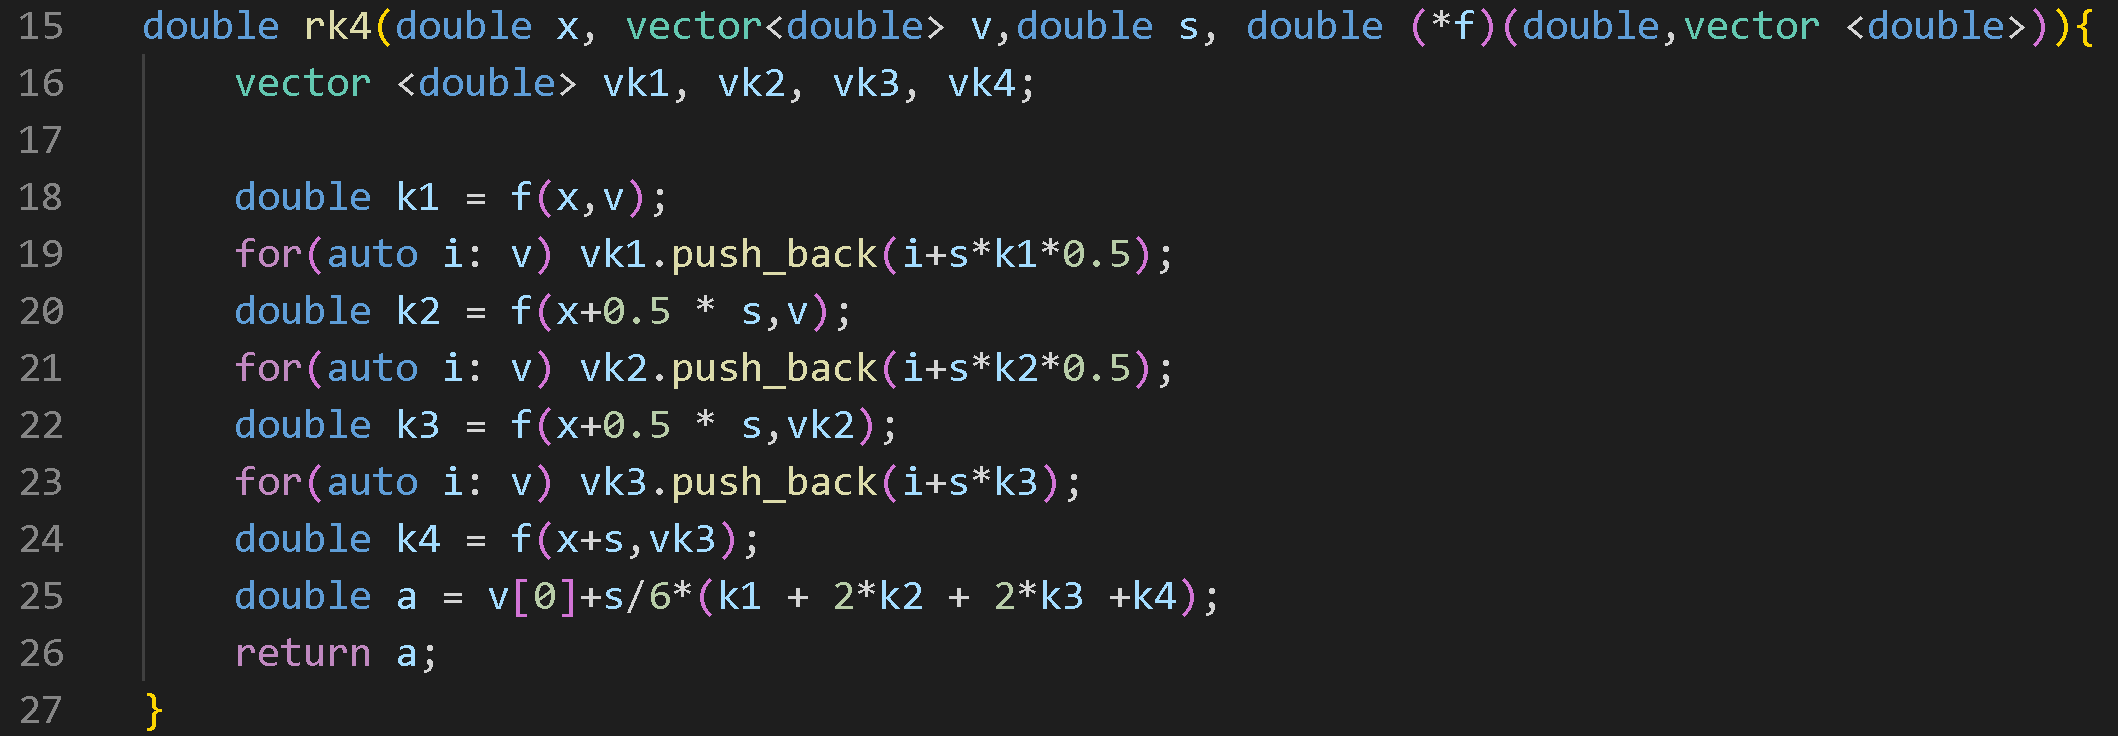
\includegraphics[width=1\textwidth]{RK4 general function}
\caption{Code implementing general RK4}
\label{fig 6}
\end{figure}
\pagebreak

We can then create 2 seperate functions for the angular acceleration of bob1 and bob2 and create a new function calling both functions seperately.

The following graphs are of the double pendulum when it starts to an intial angle of 30 degrees each.
\begin{figure}[h]
\center
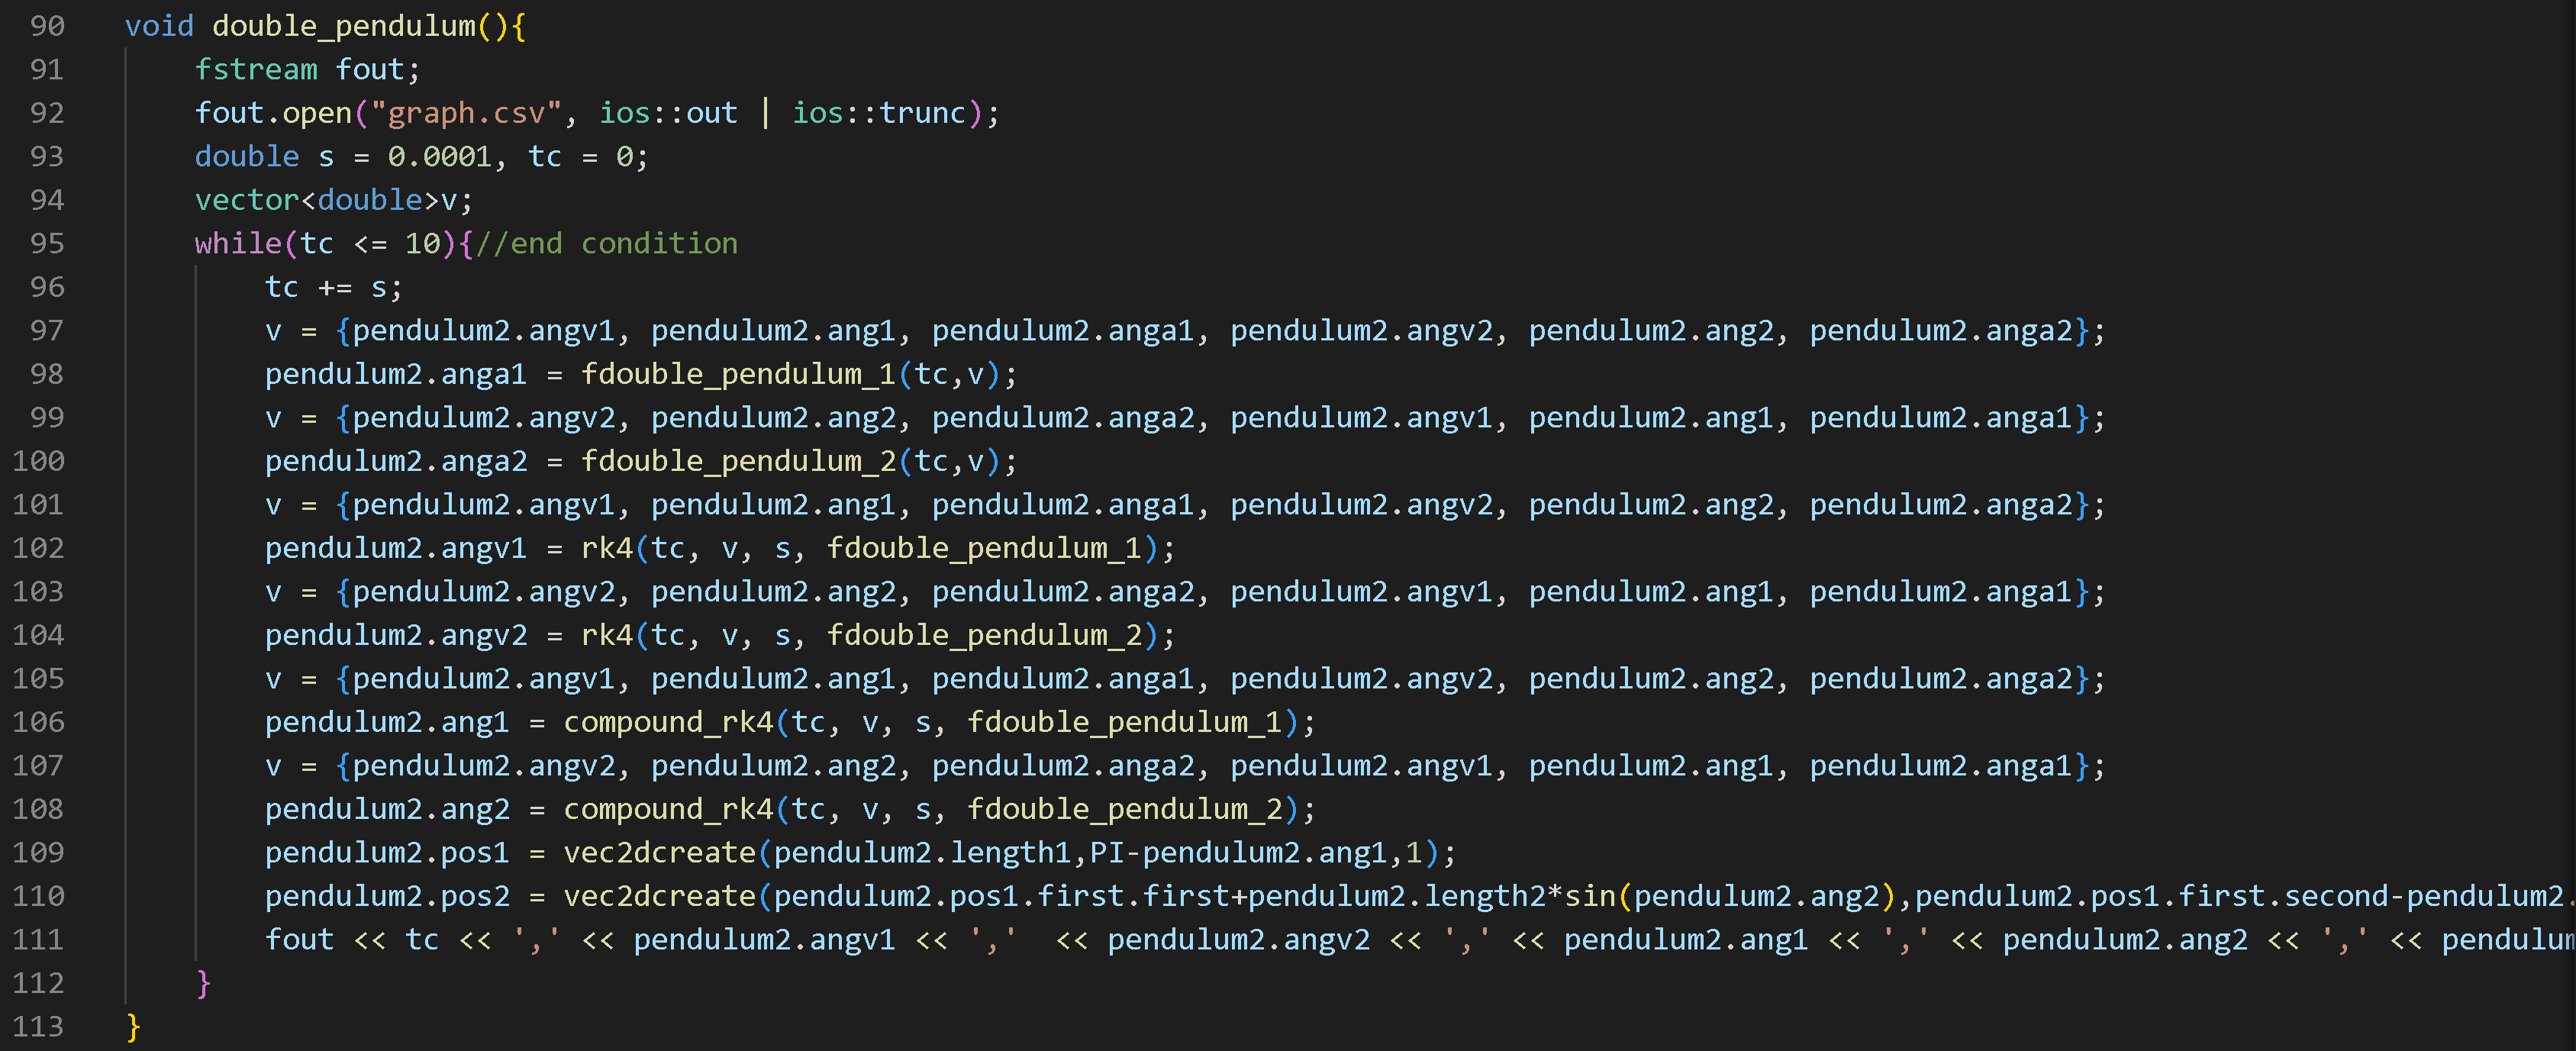
\includegraphics[width=1\textwidth]{Double pendulum function}
\caption{Code implementing general Double pendulum}
\label{fig 7}
\end{figure}
\pagebreak
\begin{figure}[h]
\center
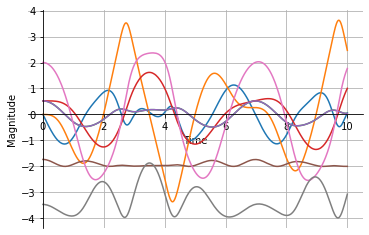
\includegraphics[width=0.625\textwidth]{Double pendulum graph}
\caption{Graph of double pendulum function}
\label{Graph 5}
\end{figure}
\begin{figure}[h]
\center
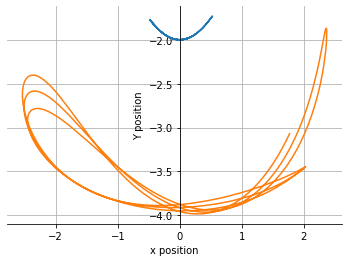
\includegraphics[width=0.625\textwidth]{Double pendulum movement graph}
\caption{Graph of movement from double pendulum graph}
\label{Graph 6}
\end{figure}
\pagebreak

\section{Conclusion}
A physics simulator can be used for many things and the physics simulator i have built can be further advanced to add constraints and to make it more general so that i can be applied to more complex systems with many more objects.

The code of my physics engine can be found at https://github.com/cadenlyy/Physics-Engine.

\section{Reflection}
This article focuses much on the software and mathematics used to simulate physics. It attempts to show the applications of such engines in analysis of physics. However, this engine could be made more generic through constrains and generalising the functions used. This would allow creation of more complex systems with ease as it would allow one to simply create an object and define it initial conditions to simulate the system. 

This system could also have been made more reader freindly by using diagrams and psuedo code in explainations as it is easier to read than C++. I could also have added a graphical interface to allow better demonstration on how the system moves instead of simply using graphs. Further more, I could also have included a comparison between the use of RK4 and Eular's intergration to show the difference instead of simply explaining it qualitatively. 

I first started writing with physics engine in January and then adapted it to fit this portflio. This project took me a good 6 months to finish as through it i learned many new things such as RK4, how to use and calculate lagraingians, what constrains are and so on. This project was somewhat of a personal interest and i had a lot of fun learning how to create a physics engine through watching videos and reading articles.

\section{References}
Davide Marenduzzo, University of Edinburgh. 
https://www2.ph.ed.ac.uk/~dmarendu/MVP/DoublePendulumTutorial.pdf

\end{document}